%!TEX program = xelatex
\documentclass[12pt]{article}

% ---------- IDIOMA ----------
% --- Paquetes para XeLaTeX y codificación moderna ---
\usepackage{fontspec} 
\usepackage[spanish, es-tabla]{babel} 
% --- Cambiar "Cuadro" por "Tabla" ---
\addto\captionsspanish{\renewcommand{\tablename}{Tabla}}

% ---------- FUENTES ----------
\setmainfont{TeX Gyre Termes}

% ---------- PAQUETES MATEMÁTICOS Y FÍSICOS ----------
\usepackage{amsmath,amssymb}
\usepackage{amsfonts}
\usepackage{physics}

% ---------- GRÁFICOS Y COLORES ----------
\usepackage{xcolor}
\usepackage{graphicx}
\usepackage{tikz}
\usetikzlibrary{babel} % <- Agrega esta línea
\usepackage{tikz-3dplot}
\usetikzlibrary{shapes, arrows, positioning, calc}
\usetikzlibrary{arrows.meta} 
\usetikzlibrary{shapes.geometric} 
\usetikzlibrary{decorations.markings}

% ---------- CÓDIGO (LISTINGS) ----------
\usepackage{listings}
\usepackage{lastpage}

\definecolor{codegreen}{rgb}{0,0.6,0}
\definecolor{codegray}{rgb}{0.95,0.95,0.95}
\definecolor{codepurple}{rgb}{0.58,0,0.82}
\definecolor{backcolour}{rgb}{0.96,0.96,0.96}

\lstdefinestyle{pythonstyle}{
    backgroundcolor=\color{backcolour},   
    commentstyle=\color{codegreen},
    keywordstyle=\color{magenta},
    numberstyle=\tiny\color{gray},
    stringstyle=\color{codepurple},
    basicstyle=\ttfamily\small,          
    breakatwhitespace=false,         
    breaklines=true,                     
    captionpos=b,                    
    keepspaces=true,                 
    numbers=left,                        
    numbersep=5pt,                  
    showspaces=false,                
    showstringspaces=false,
    showtabs=false,                  
    tabsize=4,
    language=Python                      
}
\lstset{style=pythonstyle}

% ---------- DISEÑO Y ESTILO ----------
\usepackage{geometry}
\geometry{letterpaper, margin=2cm, headheight=15pt}
\usepackage{fancyhdr} 
\usepackage{lastpage} 
\usepackage{wrapfig}
\usepackage{multicol}
\usepackage{enumitem}
\usepackage{framed}
\usepackage{etoolbox}

% ---------- TCOLORBOX ----------
\usepackage[most,skins,theorems]{tcolorbox}

% --- Caja para Definiciones Formales ---
\newtcolorbox{definicion}[1][]{
  enhanced,
  breakable, 
  colback=blue!5!white,
  colframe=blue!75!black,
  fonttitle=\bfseries,
  title={Definición: #1},
  arc=2mm,
  boxrule=0.8pt,
  drop shadow=black!10!white
}

% --- Caja para Tareas ---
\newtcolorbox{problemas}[1][]{
  enhanced,
  breakable, 
  colback=violet!6!white,       
  colframe=violet!45!white,     
  coltitle=violet!40!black,     
  fonttitle=\bfseries,
  title={Problemas: #1},
  arc=2.5mm,                    
  boxrule=0.8pt,
  drop shadow=black!8!white     
}

% --- Caja Libre Verde Menta ---
\newtcolorbox{cajaflex}[1][]{
  enhanced,
  breakable, 
  colback=teal!5!white,       
  colframe=teal!50!black,     
  coltitle=teal!10!white,     
  fonttitle=\bfseries,
  code={\ifblank{#1}{}{\tcbset{title={#1}}}},
  arc=2.5mm,                  
  boxrule=0.8pt,
  drop shadow=black!8!white   
}

% ---------- TABLAS Y ELEMENTOS EXTRA ----------
\usepackage{booktabs}   
\usepackage{pifont}     
\usepackage{array}      
\usepackage{caption}    
\newcommand{\lapiz}{\ding{46}\ }

% ---------- ENLACES Y PDF ----------
\usepackage{hyperref}

\definecolor{myblue}{RGB}{20, 20, 120}
\definecolor{myred}{RGB}{220, 30, 30}
\definecolor{mygreen}{RGB}{0, 130, 60}

% Personalización de nombres para \autoref
\def\tableautorefname{Tabla}
\def\figureautorefname{Figura}
\def\equationautorefname{Ecuación}
\def\sectionautorefname{Sección}

% ---------- CONFIGURACIÓN DE ENCABEZADOS (ITM) ----------
\newcommand{\logo}{
\includegraphics[height=3cm]{escudoitm}}
\newcommand{\escola}{Facultad de Ciencias Exactas y Aplicadas}
\newcommand{\disc}{Física Computacional 1}
\newcommand{\auth}{Robinson Longas Bedoya}
\newcommand{\emaill}{\url{robinsonlongas@itm.edu.co}}
\newcommand{\email}{\url{robinsonlongas3586@correo.itm.edu.co}}
\newcommand{\cabec}{Física Computacional 1}

\hypersetup{
    colorlinks=true,
    linkcolor=blue,
    urlcolor=blue,
    citecolor=blue,
    pdftitle={\cabec\ -- \auth},
    pdfauthor={\auth}
}

% Configuración de estilos de página
\pagestyle{fancy}
\fancyhf{} 

\fancypagestyle{firstpage}{
    \fancyhead[L]{\logo}
    \fancyhead[R]{
        \textsf{\escola \\} 
        \textsf{\disc \\}
        \textsf{\auth \\}
        \textsf{\email \\} 
        \textsf{\emaill}     
    }
    \fancyfoot[R]{\scriptsize Página \thepage~de \pageref{LastPage}}
    \renewcommand{\headrulewidth}{0pt} 
    \renewcommand{\footrulewidth}{0.4pt} 
}

\fancyhead[L]{\textsf{\scriptsize \cabec\ -- \auth\ -- \email\ -- \emaill}}
\fancyfoot[R]{\scriptsize Página \thepage~de \pageref{LastPage}}
\renewcommand{\headrulewidth}{0.4pt} 
\renewcommand{\footrulewidth}{0.4pt} 

\setlength{\parskip}{0.3em}

\begin{document}
		\thispagestyle{firstpage}
		\vspace*{1.5cm}
	
	\begin{center}
		\rule{\textwidth}{0.4pt}
	\end{center}
	
	\begin{itemize}[leftmargin=*,label=\textcolor{red}{\ensuremath{\blacktriangleright}}]
		\item \textbf{Lectura y escritura de archivos}
	\end{itemize}
	
	\noindent
	\textbf{\underline{Bibliografía}}
	\begin{itemize}[leftmargin=*, label={\textcolor{blue}{$\bullet$}}]
		\item \textit{Computational Physics, Capítulo 2}, Mark Newman.
		\item \textit{Introducción a la programación con Python. Capítulo 8}, Andrés Marzal, Isabel Gracia y Pedro García.
        \item \textit{Programming for computations- Python. Sección: 5.5}, Evein Linge and Petter Langtangen. 
        \item \textit{Computational Physics with Python. Capítulo 0}, Eric Ayars. 
    \end{itemize}
     
\section*{\textcolor{red}{\textit{Entrada y salida de datos: Lectura y escritura de archivos}}}

La interacción con archivos de texto para la lectura de datos de entrada y la 
exportación de resultados es una tarea fundamental en el cálculo científico y la física 
computacional.

\subsection*{1. La función \texttt{open()} y Modos de Apertura}

Para trabajar con un archivo en Python, primero debemos abrirlo mediante la función 
integrada \texttt{open()}, la cual recibe el nombre del archivo y el modo de acceso:

\begin{itemize}
    \item \texttt{'r'} (\textit{Read}): Abre el archivo para lectura (modo por defecto). Genera un error si el archivo no existe.
    \item \texttt{'w'} (\textit{Write}): Abre el archivo para escritura. Sobrescribe completamente el contenido si el archivo ya existe o lo crea si no existe.
    \item \texttt{'a'} (\textit{Append}): Abre el archivo para anexar datos al final sin modificar el contenido preexistente.
\end{itemize}

\subsection*{2. El Gestor de Contexto (\texttt{with})}

En el Python moderno, las operaciones de entrada/salida se gestionan mediante la 
sentencia \texttt{with}. Esto garantiza la liberación adecuada de los recursos del sistema (como los descriptores de archivo) de forma automática al salir del bloque, incluso si ocurren excepciones durante la ejecución:

\begin{lstlisting}[language=Python]
with open('archivo.txt', 'r') as f:
    # Bloque de operacion sobre el archivo
    pass
# El archivo se cierra automaticamente aqui
\end{lstlisting}

\subsection*{3. Operaciones Básicas de Lectura y Escritura}

A continuación se detallan los métodos elementales para la manipulación de información en disco:

\begin{itemize}
    \item \textbf{Lectura línea a línea (\texttt{readline()}):} Devuelve una sola cadena de texto correspondiente a la línea actual y avanza el cursor interno.
    \item \textbf{Iteración directa sobre el flujo:} Recorrer directamente el objeto de archivo mediante un bucle \texttt{for} permite procesar archivos de gran tamaño de manera altamente eficiente en memoria RAM.
    \item \textbf{Escritura (\texttt{write()}):} Escribe una cadena de texto en el archivo. Requiere incluir explícitamente el carácter de salto de línea (\texttt{\textbackslash n}) al final de cada registro.
\end{itemize}

\subsection*{\textcolor{blue}{\textit{Ejemplo:}}}
Consideremos como ejemplo un archivo de entrada \texttt{masavolumen.txt} que contiene la información de la Tabla~\ref{tab:datos_entrada}:

\begin{table}[h!]
\centering
\begin{tabular}{cc}
\toprule
\textbf{Masa (g)} & \textbf{Volumen (m$^3$)} \\
\midrule
1000000 & 1 \\
500000 & 0.1 \\
300000 & 0.2 \\
\bottomrule
\end{tabular}
\caption{Tabla con valores para la masa y el volumen de un cuerpo.}
\label{tab:datos_entrada}
\end{table}

El siguiente programa lee las variables, massa y volumen, 
calcula la densidad ($\rho = m/V$) y genera un nuevo archivo \texttt{resultados.txt}:

\begin{lstlisting}[language=Python, captionpos=t, title=\texttt{in\_out.py}]
"""En este programa se ilustra el uso de la lectura y la escritura de ficheros"""

archivo_entrada='masavolumen.txt'
archivo_salida='masavolumendensidad.txt'

#abrimos los archivos
with open(archivo_entrada, 'r') as f_in, open(archivo_salida, 'w') as f_out:
    # 1. Leer y escribir el encabezado
    encabezado = f_in.readline()
    f_out.write(f"{encabezado.strip()}   Densidad (g/m^3)\n")
    
    # 2. Procesar linea a linea
    for linea in f_in:
        partes = linea.split()
        if partes:  # Omite lineas vacias
            masa = float(partes[0])
            volumen = float(partes[1])
            densidad = masa / volumen
            
            # 3. Guardar resultados 
            f_out.write(f"{masa:<10.1f} {volumen:<10.2f} {densidad:<12.2f}\n")
\end{lstlisting}

\subsection*{\textcolor{blue}{\textit{Ejemplo: masa inercial vs masa gravitacional}}}

En el contexto de la interacción gravitacional, se tiene que la interacción entre dos cuerpos 
de masas gravitacionales $m_g$ y $M_g$ está dictaminada por la \textit{ley de gravitación universal}
$$F = -G\frac{m_gM_g}{r^2}\,,$$ donde $G$ es la constante de newton y $r$ la separación entre las
masas. Por otro lado, la ley de inercia de Galileo-Newton, implica que $F = m_i a$, donde 
$m_i$ es la masa inercial que representa la "resistencia" de un cuerpo a cambiar su estado 
de movimiento.

Conceptualmente, la masa inercial y gravitacional son diferentes, sin embargo, el 
experimento muestra que hay una relación entre ellas, $m_i=m_g$, lo que constituye
un principio fundamental en la teoría de la relatividad general, \textit{el principio de
equivalencia}.

Para el caso de un péndulo de longitd $l$ que oscila con un periodo $T$, se puede mostrar
que $\dfrac{m_g}{m_i}= 4.02811 \dfrac{l}{T^2}$. En el archjivo \lstinline|datosL1.txt|
se encuentran los datos experimentales medidos pra $l$ y $T$. En el sigueinte programa, se leen 
esos datos y se calcula la razpkn entra la masa inercial y gravitacional.

\begin{lstlisting}[language=Python, captionpos=t, title=\texttt{masaIvsmasaG.py}]
"""En este programa se ilustra el uso de la lectura de datos para graficarlos"""
import numpy as np
import matplotlib.pyplot as plt

datos= np.loadtxt('datosL1.txt')
l = datos[:,0] # la primera columna es la longitud
t = datos[:,1] # la segunda columna es el tiempo
#calculo de la masa gravitacional/ masa inercial
mgmi = 4.0281 * l / (t**2)

# plot
plt.figure(figsize=(8, 6))
plt.plot(t, mgmi, color='red', ls='-', lw=3, label=r'$\boldsymbol{Datos}$')
plt.yscale('log')
plt.ylim(0.1,10)
plt.axhline(1, color='black', ls='--', lw=3, label=r'$\boldsymbol{Esperado}$')
plt.xlabel("tiempo(s)", size=20)
plt.ylabel(r'$\boldsymbol{m_g/m_i}$', size=20)
plt.legend(prop={'size': 15}, loc='upper left', frameon=True)
plt.savefig("mgvsmi.pdf")
plt.show()
\end{lstlisting}

\begin{figure}[htbp]
    \centering
    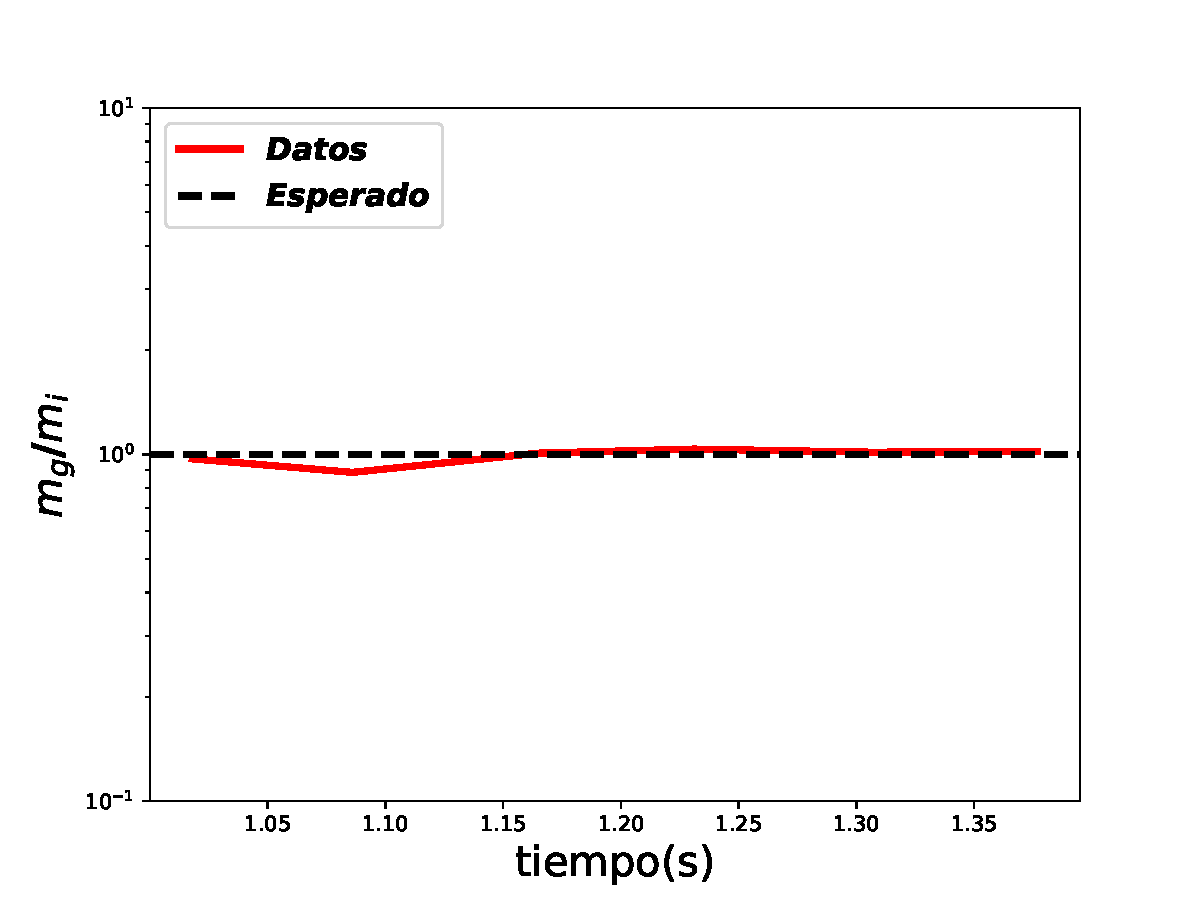
\includegraphics[width=0.65\textwidth]{mgvsmi.pdf}
    \caption{Prueba experimental del principio de equivalencia.}
\end{figure}

\subsection*{\textcolor{blue}{\textit{Ejemplo:}}}

Para finalizar, consideremos un archivo de datos experimental 
denominado \texttt{microphones.txt}, cuyo contenido está organizado por 
columnas separadas por tabulaciones o espacios:

\begin{table}[h!]
\centering
\begin{tabular}{ccc}
\toprule
\textbf{\#Frequency} & \textbf{Mic 1} & \textbf{Mic 2} \\
\midrule
10.000 & 0.654 & 0.192 \\
11.000 & 0.127 & 0.032 \\
12.000 & 0.120 & 0.030 \\
13.000 & 0.146 & 0.031 \\
14.000 & 0.155 & 0.033 \\
15.000 & 0.175 & 0.036 \\
\vdots & \vdots & \vdots \\
\bottomrule
\end{tabular}
\caption{Estructura del archivo \texttt{datosmicrofono.txt}.}
\label{tab:microphones}
\end{table}


\begin{lstlisting}[language=Python, captionpos=t, title=\texttt{microfono.py}]
import numpy as np
import matplotlib.pyplot as plt

# Cargar las columnas directamente en variables independientes
frequency, mic1, mic2 = np.loadtxt('datosmicrofono.txt', unpack=True)

# graficar
plt.figure(figsize=(8, 5))
plt.plot(frequency, mic1, 'r-', label='Micrófono 1')
plt.plot(frequency, mic2, 'b-', label='Micrófono 2')

plt.xlabel('Frecuencia (Hz)',size=15)
plt.ylabel('Amplitud (cm)',size=15)
plt.legend(loc='upper right')
plt.grid(True, ls=':', alpha=0.6)
plt.savefig("../Clases/Introduccion_Python/microfono.pdf")
plt.show()
\end{lstlisting}

\begin{figure}[htbp]
    \centering
    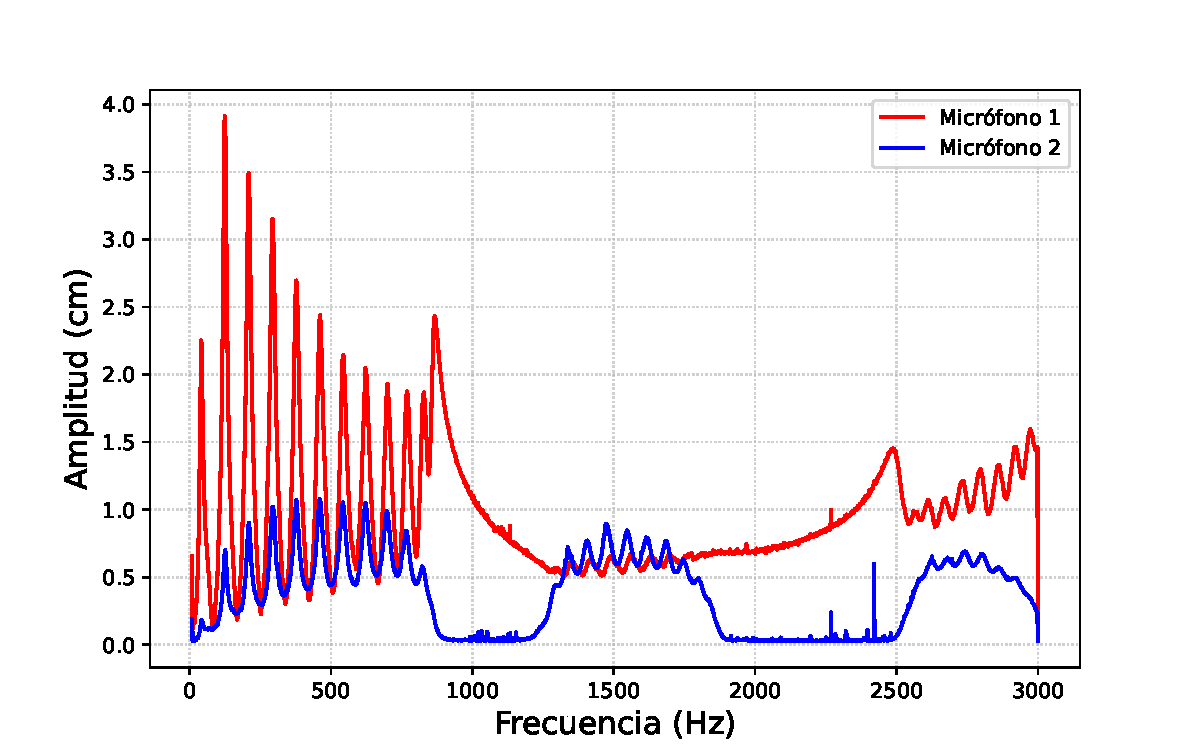
\includegraphics[width=0.8\textwidth]{microfono.pdf}
   \caption{Datos de los micrófonos.} 
   \label{fig:micro}
\end{figure}

\begin{itemize}
    \item \textbf{\texttt{unpack=True}} le indica a la función que el archivo contiene datos dispuestos en columnas y que debe devolver cada una de ellas como un arreglo independiente de NumPy.
    \item \textbf{\texttt{np.loadtxt()}} ignora cualquier línea que comience con el carácter \texttt{\#}, asumiendo que se trata de un encabezado o comentario.
    \item Se requiere que todas las filas tengan exactamente el mismo número 
    de columnas y que todos los elementos sean valores numéricos.
\end{itemize}

\begin{problemas}[]
\begin{enumerate}[leftmargin=*]

\item La forma más útil de analizar los datos mostrados en la \autoref{fig:micro}
es calculando la razón entre las señales de ambos micrófonos. Grafique esta razón 
($\text{Mic 1} / \text{Mic 2}$) en función de la frecuencia en el eje $x$. 
Asegúrese de dar un acabado adecuado a la gráfica ajustando las escalas, 
las etiquetas de los ejes y el título correspondiente. 
\item El archivo \texttt{radiative.txt} contiene dos columnas de datos: la primera corresponde a los conteos registrados por un contador Geiger y la segunda al tiempo en segundos.
\begin{enumerate}[label=(\alph*)]
    \item Genere una gráfica adecuada y clara de estos datos.
    \item Si los datos siguen una curva exponencial, al graficar el logaritmo natural de los conteos (o al representar los datos originales en una escala semilogarítmica) se debería obtener una línea recta. Determine si este es el caso y explique su conclusión respaldándola con una gráfica apropiada.
\end{enumerate}
\item Los datos en el archivo \texttt{radiative.txt} 
corresponden a mediciones reales de un experimento de decaimiento radiactivo; la primera columna es el número de decaimientos $N$ y la segunda es el tiempo $t$ en segundos. Nos interesa determinar el tiempo de vida media $t_{1/2}$ del $^{137}\text{Ba}$.

El decaimiento sigue la ecuación teórica:
\[
N(t) = N_0 e^{-\lambda t} \quad \text{donde} \quad \lambda = \frac{\ln 2}{t_{1/2}}
\]

Utilizando las técnicas aprendidas en este capítulo, 
cargue los datos del archivo \texttt{radiative.txt} en 
variables adecuadamente nombradas en una sesión de Python. 
Experimente con diferentes valores de $N_0$ y $\lambda$ (o $t_{1/2}$) y 
grafique la curva teórica sobre los datos experimentales. 
Intente ajustar los valores manualmente hasta que la curva coincida 
adecuadamente con los datos. ¿Cuál es su mejor estimación para $t_{1/2}$?
\end{enumerate}

\end{problemas}

\end{document}

